\chapter{Background and Related Work}
\label{ch:background}

This chapter summarizes the modeling and systems context needed to understand a SimLingo-style VLA driving policy, and motivates why simulator-to-simulator transfer is non-trivial even when both platforms provide similar sensors and control APIs.

\section{Two-level autonomous driving architecture}
\label{sec:two-level}
Learned driving systems typically separate the problem into two levels. The \emph{upper level} is a learned policy that takes sensor data (camera images) and route intent (e.g., a target-point coordinate) and predicts a future trajectory as a sequence of waypoints in the vehicle's ego frame. The \emph{lower level} is a classical controller that converts these waypoints into low-level actuator commands---steering angle and throttle/brake---using PID control loops.

\begin{figure}[ht]
\centering
\resizebox{\textwidth}{!}{%
\begin{tikzpicture}[
  block/.style={draw, rounded corners, minimum height=1.1cm, minimum width=2.2cm,
                align=center, font=\small},
  arrow/.style={-{Stealth[length=2.5mm]}, thick},
  lbl/.style={font=\scriptsize, midway},
  annot/.style={draw=gray!60, dashed, rounded corners=2pt, inner sep=3pt,
                font=\scriptsize, align=left, fill=gray!5},
]
  % === Camera frame (actual QLabs image) ===
  \node[inner sep=1pt, draw, thin] (img) at (0,0)
    {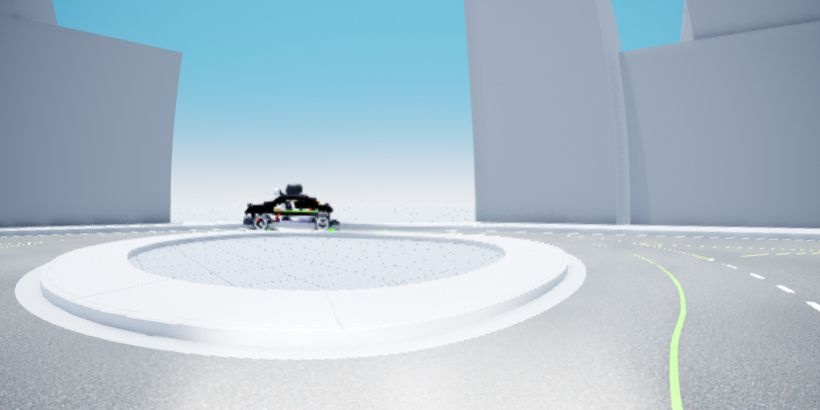
\includegraphics[width=2.8cm]{figures/qlabs_frame_0072.jpg}};

  % === Vision Encoder ===
  \node[block, fill=blue!10, right=0.8cm of img] (vision)
    {Vision\\Encoder\\[-2pt]{\scriptsize InternViT-300M}};

  % === Language Model ===
  \node[block, fill=blue!10, right=2.0cm of vision] (llm)
    {Language\\Model\\[-2pt]{\scriptsize Qwen2-0.5B}};

  % === PID controllers ===
  \node[block, fill=orange!10] (lateral) at (12.0,1.2) {Lateral PID};
  \node[block, fill=orange!10] (speed) at (12.0,-1.4) {Speed\\Controller};

  % === Vehicle ===
  \node[block, fill=green!10] (vehicle) at (16.0,0) {QCar~2};

  % === Nav conditioning input (below LLM, shifted left) ===
  \node[annot, below=1.8cm of llm, xshift=-1.0cm] (nav)
    {$v = 2.15\;\text{m/s}$\\[1pt]$\mathbf{tp} = (15.16,\; 31.45)$};

  % === Arrows: camera to vision encoder ===
  \draw[arrow] (img) -- (vision);

  % === Arrow: vision encoder to LLM (with token notation) ===
  \draw[arrow] (vision) -- node[lbl, above]
    {$\mathbf{e}_I \in \mathbb{R}^{512 \times 896}$} (llm);

  % === Arrow: nav input to LLM ===
  \draw[arrow] (nav) -- (llm);

  % === LLM to PID (split outputs) ===
  \draw[arrow] (llm.east) ++(0,0.1) -- (lateral.west);
  \draw[arrow] (llm.east) ++(0,-0.1) -- (speed.west);

  % === Route WP annotation box (label + data, above the route arrow) ===
  \node[annot] (rwp) at ($(llm.east)!0.5!(lateral.west) + (0.5,2.5)$)
    {\textit{20 route waypoints}\\[2pt]
     $\mathbf{w}_0{=}(0.02,\; 0.01)$\\[1pt]
     $\mathbf{w}_1{=}(0.89,\; 0.02)$\\[1pt]
     $\;\;\vdots$\\[-2pt]
     $\mathbf{w}_{19}{=}(16.75,\; {-}3.16)$};
  \draw[-{Stealth[length=1.5mm]}, gray, thin]
    (rwp.south) -- ($(llm.east)!0.5!(lateral.west) + (0,0.65)$);

  % === Speed WP annotation box (label + data, below the speed arrow) ===
  \node[annot] (swp) at ($(llm.east)!0.5!(speed.west) + (0.5,-2.6)$)
    {\textit{10 speed waypoints}\\[2pt]
     $\mathbf{s}_0{=}(0.40,\; 0.00)$\\[1pt]
     $\;\;\vdots$\\[-2pt]
     $\mathbf{s}_9{=}(3.69,\; {-}0.80)$};
  \draw[-{Stealth[length=1.5mm]}, gray, thin]
    (swp.north) -- ($(llm.east)!0.5!(speed.west) + (0,-0.65)$);

  % === PID to vehicle ===
  \draw[arrow] (lateral.east) -- node[lbl, above]
    {$\delta = \frac{\pi}{9} \approx 20^\circ$} (vehicle.west |- lateral.east);
  \draw[arrow] (speed.east) -- node[lbl, below, pos=0.55]
    {$v_{\text{cmd}} = 2.33$ m/s} (vehicle.west |- speed.east);

  % === Level separator ===
  \draw[dashed, gray] (8.8,-4.0) -- (8.8,4.5);
  \node[font=\scriptsize\itshape, gray] at (3.5,4.2)
    {Upper level (learned)};
  \node[font=\scriptsize\itshape, gray] at (14.0,4.2)
    {Lower level (classical)};
\end{tikzpicture}%
}% end resizebox
\caption[Two-level driving architecture with QLabs data.]{Two-level driving architecture instantiated with QLabs data. The camera input shows a QLabs roundabout scene; the vision encoder (InternViT-300M) produces $512$ visual tokens projected to the language model's $896$-dimensional embedding space. The language model (Qwen2-0.5B) predicts $20$ route waypoints and $10$ speed waypoints in the ego frame (example values from a representative inference step at $v = 2.15$\,m/s). Classical PID controllers convert waypoints to steering ($\delta_{\max} = \pi/9$) and velocity commands.}
\label{fig:two-level}
\end{figure}

This separation means the learned model never directly outputs steering or throttle values---it only predicts \emph{where} the vehicle should go. The PID controllers then determine \emph{how} to get there. This decoupling simplifies the learning problem and makes the controller independently tunable.

\section{Vision--Language--Action models}
Modern Vision-Language models commonly pair (i) a vision encoder that converts an image into a sequence of visual tokens with (ii) a large language model (LLM) that consumes text tokens, plus (iii) a learned projection that maps vision features into the LLM embedding space. In this formulation, actions can be represented as text (e.g., tokens describing a maneuver), as continuous vectors regressed from hidden states (the internal vector representations a transformer produces for each token at its final layer), or as structured outputs such as future waypoints.

Driving is a particularly natural application for VLA systems because navigation intent is often compact and language-like (``follow the road'', ``turn left''), while the environment context is high-dimensional and visual. The key systems challenge is that the policy must run in closed loop, meaning perception, prompt construction, inference, and control must all execute reliably at a fixed cadence.

\section{Imitation learning}
Imitation learning (IL) learns a policy from expert demonstrations \citep{pomerleau1988alvinn,bojarski2016end}. In simulation, the expert can be a scripted controller, a human teleoperator, or a privileged planner. A core IL consideration is \emph{train--inference mismatch}: if the policy observes a slightly different state distribution at inference than during data collection, errors can compound over time \citep{ross2011dagger}. This mismatch is amplified when transferring across simulators because sensor models, coordinate conventions, and dynamics differ.

\section{SimLingo}
\label{sec:simlingo}
SimLingo is a vision-language-action (VLA) model for closed-loop autonomous driving that unifies waypoint prediction with natural-language generation \citep{simlingo2023}. It was the winning entry of the CARLA Autonomous Driving Challenge~2024 and achieves state-of-the-art performance on the Bench2Drive benchmark \citep{jia2024bench2drive}. The following subsections describe its architecture in detail; the adaptation of this architecture to QLabs is the subject of \Cref{ch:methodology,ch:training,ch:inference}.

\subsection{Backbone model: InternVL2-1B}
\label{sec:internvl2}
SimLingo is built on top of \texttt{OpenGVLab/InternVL2-1B} \citep{internvl2}, a multimodal vision--language model comprising two main components:
\begin{itemize}[leftmargin=*,itemsep=0.25em]
  \item \textbf{Vision encoder}: InternViT-300M-448px, a 300\,M-parameter vision transformer \citep{dosovitskiy2021vit} pretrained at $448\times448$ resolution.
  \item \textbf{Language model}: Qwen2-0.5B-Instruct, a 500\,M-parameter causal language model \citep{yang2024qwen2}.
\end{itemize}
A learned projection layer maps the vision encoder's output features into the language model's embedding space, enabling the LLM to process both visual and textual tokens in a single forward pass. In practice, the choice of InternVL2-1B affects (i)~the image tokenization scheme, (ii)~the conversation template formatting, and (iii)~the compute and memory requirements for fine-tuning.

\subsection{Vision encoder and image tokenization}
\label{sec:vision-encoder}
To handle input images at higher resolution than the pretrained $448\times448$ patch size, InternVL2 uses \emph{dynamic tiling}: each input image is split into $N_I$ non-overlapping $448\times448$ tiles that are encoded independently by InternViT. A pixel-unshuffle downsampling step ($\rho$, factor of~4) then reduces the token count, representing each tile by 256~visual tokens. With $N_I{=}2$ tiles (the configuration used in this work), the vision encoder produces $512$~visual tokens total:
\begin{equation}
  \mathbf{e}_I \in \mathbb{R}^{(N_I \cdot 256)\times D},
\end{equation}
where $D$ is the embedding dimension of the language model. This tiling strategy reuses the pretrained encoder without retraining at a different resolution.

\subsection{Navigational conditioning}
\label{sec:nav-conditioning}
SimLingo supports two navigation modes that provide the model with route intent:
\begin{enumerate}[leftmargin=*,itemsep=0.25em]
  \item \textbf{Target-point mode.} Two GPS-like waypoint coordinates are fed through a learned MLP (the \texttt{WaypointInputAdaptor}: $\text{Linear}(2{\to}256) \to \text{ReLU} \to \text{Linear}(256{\to}512) \to \text{ReLU} \to \text{Linear}(512{\to}D)$), producing two navigational embeddings $\mathbf{e}_{\text{nav}} \in \mathbb{R}^{2\times D}$ that replace \texttt{<TARGET\_POINT>} placeholder tokens in the prompt.
  \item \textbf{Command mode.} A high-level command string (e.g., ``turn left at the next intersection'') is tokenized by the standard LLM tokenizer, producing variable-length navigational embeddings $\mathbf{e}_{\text{nav}} \in \mathbb{R}^{N_{\text{HLC}}\times D}$.
\end{enumerate}
During training, the original SimLingo randomly switches between modes to learn from both geometric and language-based conditioning. This work uses target-point mode exclusively; the rationale is discussed in \Cref{ch:training}.

\subsection{Prompt construction and token interleaving}
\label{sec:prompt-construction}
All inputs are assembled into a single global prompt:
\begin{quote}
\texttt{<IMG\_CONTEXT>$\backslash$n Current speed: <v>m/s. Command: <TARGET\_POINT><TARGET\_POINT>. <task prompt>.}
\end{quote}
A \emph{token interleaver} (IL) replaces placeholder tokens in this prompt with actual embeddings: visual tokens at \texttt{<IMG\_CONTEXT>}, waypoint embeddings at \texttt{<TARGET\_POINT>}, and learnable action query tokens at the end. Let $\mathbf{e}_L$ denote the text token embeddings produced by the LLM embedding layer from the tokenized prompt, $\mathbf{e}_I$ the visual token embeddings from the vision encoder (which replace \texttt{<IMG\_CONTEXT>} placeholders in $\mathbf{e}_L$), and $\mathbf{e}_{\text{nav}}$ the navigational embeddings produced by the \texttt{WaypointInputAdaptor} (which replace \texttt{<TARGET\_POINT>} placeholders). The resulting unified sequence
\begin{equation}
  \mathbf{e}_{\text{LLM}} = \text{IL}(\mathbf{e}_L,\; \mathbf{e}_I,\; \mathbf{e}_{\text{nav}})
\end{equation}
is passed to the language model alongside learnable \emph{action query tokens} $\mathbf{q}_{\text{route}}$ and $\mathbf{q}_{\text{speed}}$:
\begin{equation}
  [\mathbf{o}_l,\; \mathbf{o}_{\text{route}},\; \mathbf{o}_{\text{speed}}] = \text{LLM}([\mathbf{e}_{\text{LLM}},\; \mathbf{q}_{\text{route}},\; \mathbf{q}_{\text{speed}}]).
\end{equation}
Here $\mathbf{q}_{\text{route}}$ consists of 20~learnable vectors (one per route waypoint to predict) and $\mathbf{q}_{\text{speed}}$ consists of 10~learnable vectors (one per speed waypoint). These are randomly initialized parameters (\texttt{nn.Parameter}) that are appended after the prompt tokens so the transformer can attend over the full visual-linguistic context. After the forward pass, the hidden states at each query position are decoded by an MLP head into 2-D ego-frame coordinate deltas; cumulative summation converts the deltas to absolute waypoint positions. For example, a concrete input sequence looks like:

\medskip
\noindent\texttt{\small <system> Current speed: 2.5\,m/s. <img>[512 visual tokens]</img> Target: [nav$_1$(x,y)][nav$_2$(x,y)]. Predict the waypoints. <assistant> Waypoints: $|$ $\mathbf{q}_{\text{route}} \times 20$ $|$ $\mathbf{q}_{\text{speed}} \times 10$}
\medskip

SimLingo defines four task prompts: (i)~driving-only (``Predict the waypoints''), (ii)~commentary (``What should the ego do next?''), (iii)~visual question answering, and (iv)~action dreaming (counterfactual instructions). This work uses only the driving-only prompt.

\subsection{Dual-head action prediction}
\label{sec:dual-head}
SimLingo uses a \emph{disentangled} action representation with two complementary waypoint outputs, each predicted non-autoregressively from the LLM's hidden states via learnable query tokens:
\begin{itemize}[leftmargin=*,itemsep=0.25em]
  \item \textbf{Speed waypoints} (temporal): future ego-frame coordinates sampled at $0.25\,\text{s}$ intervals. These capture the vehicle's intended speed profile and are used for longitudinal (throttle/brake) PID control.
  \item \textbf{Path waypoints} (geometric): future ego-frame coordinates sampled at ${\sim}1\,\text{m}$ intervals along the predicted route. These provide denser geometric supervision and drive the lateral (steering) PID controller.
\end{itemize}
Each head applies an MLP on top of the LLM output features. The route head uses $\text{Linear}(H{\to}512) \to \text{SiLU} \to \text{Linear}(512{\to}256) \to \text{SiLU} \to \text{Linear}(256{\to}2)$; the speed head is smaller: $\text{Linear}(H{\to}256) \to \text{SiLU} \to \text{Linear}(256{\to}2)$, where $H$ is the LLM hidden size. Both MLPs output waypoint \emph{deltas} that are converted to absolute positions via cumulative summation. The separation into temporal and geometric heads prevents the single-head trade-off between speed accuracy and steering precision observed in prior work.

\subsection{Language generation head}
In addition to action prediction, SimLingo can autoregressively generate natural-language text from the LLM hidden states using standard next-token prediction. This enables commentary generation and visual question answering. The language head is trained with a cross-entropy loss on valid text tokens. In this work, the language head is retained during fine-tuning but is not evaluated, as no natural-language annotations were collected for QLabs (see \Cref{ch:training}).

\subsection{Training losses}
\label{sec:training-losses}
SimLingo optimizes a multi-task loss combining:
\begin{itemize}[leftmargin=*,itemsep=0.25em]
  \item \textbf{Waypoint loss}: Smooth-$\ell_1$ loss between predicted and ground-truth waypoints, applied independently to both the speed and path heads.
  \item \textbf{Route loss}: Smooth-$\ell_1$ loss on the predicted route (20~waypoints ahead).
  \item \textbf{Language loss}: Cross-entropy loss on next-token predictions, masked to valid training tokens only.
\end{itemize}
All losses are summed with equal weight. The use of Smooth-$\ell_1$ (rather than $\ell_2$) was adopted to improve training stability when combined with the action-dreaming augmentation data.

\section{Efficient fine-tuning with LoRA}
Low-Rank Adaptation (LoRA) injects trainable low-rank matrices into selected linear layers of a frozen backbone, enabling efficient fine-tuning with substantially fewer trainable parameters \citep{hu2021lora}. LoRA is particularly useful for multimodal models because the frozen vision encoder can be retained while only adapting the language-side (and any projectors) to the new domain.

In this repository, training is organized using PyTorch Lightning \citep{pytorchlightning} and accelerated with DeepSpeed ZeRO optimizations \citep{deepspeed}; hyperparameters and the relevant Hydra \citep{yadan2019hydra} configurations are recorded in \Cref{app:hyperparameters}.

\section{Simulation platforms: CARLA vs. QLabs}
CARLA is an open-source simulator widely used for autonomous driving research \citep{dosovitskiy2017carla}. Quanser QLabs is a separate simulation environment designed for education and robotics experimentation, providing a QCar~2 vehicle model and APIs for sensor acquisition and actuation.

From an adaptation perspective, important differences include:
\begin{itemize}[leftmargin=*,itemsep=0.25em]
  \item \textbf{Control-loop cadence:} model and controller assumptions about sampling rate affect PID derivatives and speed estimation.
  \item \textbf{Steering conventions:} the sign and saturation of steering may differ across simulators.
  \item \textbf{Sensor geometry:} camera intrinsics/extrinsics and field-of-view affect visual appearance and downstream behavior.
  \item \textbf{Dynamics/friction:} acceleration limits, braking behavior, and static friction can change closed-loop stability.
\end{itemize}

The methodology in \Cref{ch:methodology} frames these differences as a distribution-alignment problem: the closer the inference-time signals match the training distribution, the more reliable transfer becomes.
